
\begin{figure}[H]
\centering
%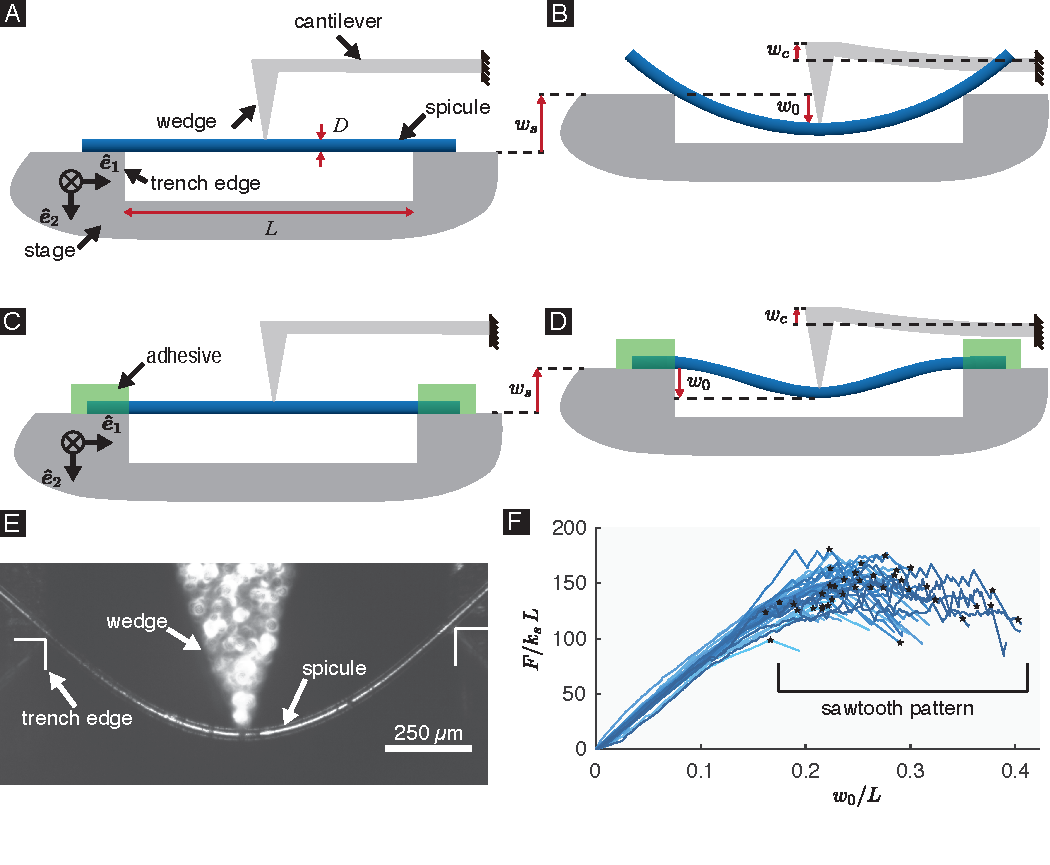
\includegraphics[width=\textwidth]{Figures/Figure3_V3.pdf}
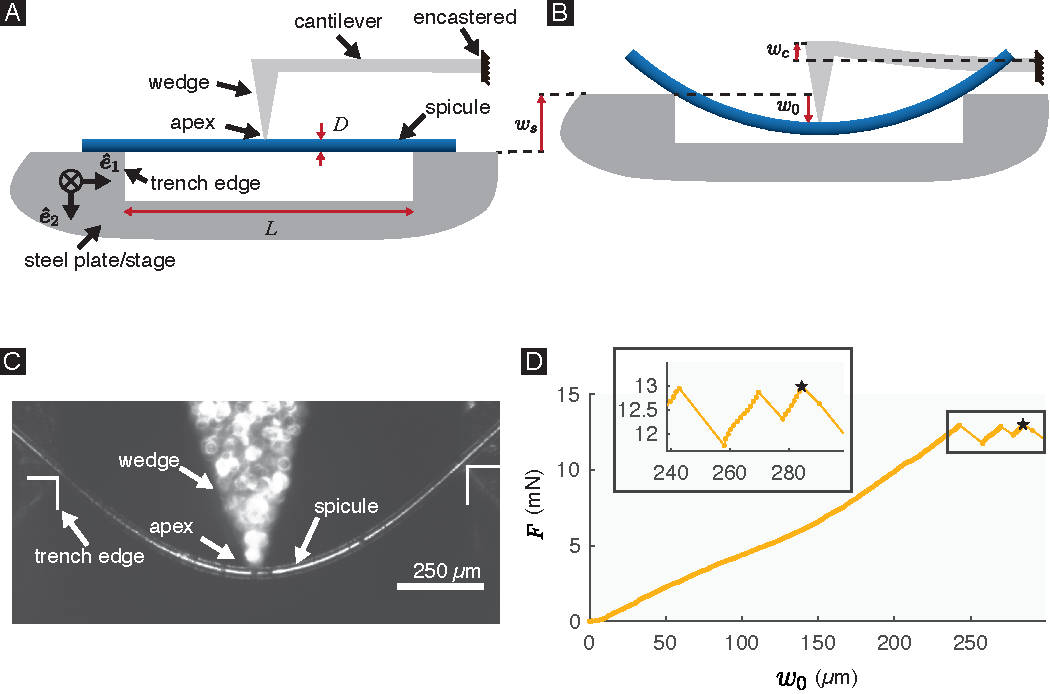
\includegraphics[width=\textwidth]{Figures/SimplySupported_V3.pdf}

\caption{
Description of three-point bending test setups and data obtained from the tests. (\textsf{A}) and (\textsf{B}) are schematics of simply-supported test setup of a spicule. The spicule is suspended over a trench, loaded at its mid span by a wedge attached to a cantilever.
Schematic (\textsf{A}) shows the reference configuration,  while schematic (\textsf{B})  shows the deformed configuration. The mid span specimen displacement, $w_0$, cantilever deflection, $w_c$, and stage displacement, $w_s$, are marked in (\textsf{A}) and (\textsf{B}).
Basis vectors $\physe_1$ and $\physe_2$ are shown in (\textsf{A}). Basis vector $\ethree$ points into the plane of the paper.
}
\label{fig:SSconfig}
\end{figure}
%\input{Comment/commentHKFig2label}
